\documentclass{article}

\usepackage[main, final]{Styles/neurips_2025}

\usepackage[utf8]{inputenc}
\usepackage[T1]{fontenc}
\usepackage{hyperref}
\usepackage{url}
\usepackage{booktabs}
\usepackage{amsfonts}
\usepackage{amsmath}
\usepackage{amssymb}
\usepackage{nicefrac}
\usepackage{microtype}
\usepackage{xcolor}
\usepackage{graphicx}
\usepackage{subcaption}
\usepackage{enumitem}
\usepackage{multirow}

\setlength{\textfloatsep}{6pt plus 2pt minus 2pt}
\setlength{\floatsep}{6pt plus 2pt minus 2pt}
\setlength{\intextsep}{6pt plus 2pt minus 2pt}
\setlength{\abovecaptionskip}{4pt}
\setlength{\belowcaptionskip}{2pt}

\title{Measuring Noise-Level Dependence in Conditional Image Generation}

\author{%
  Qile Zhang \\
  Department of ECE \\
  University of California, San Diego \\
  \texttt{qiz092@ucsd.edu} \\
  \And
  Wuxi Chen \\
  Department of ECE \\
  University of California, San Diego \\
  \texttt{wuchen@ucsd.edu} \\
}

\begin{document}
\maketitle

% ===========================================================================
\begin{abstract}
We study how the effectiveness of conditioning in diffusion models depends on noise level during inference. Through controlled inference-time interventions and quantitative diagnostics, we analyze how both \emph{text} and \emph{structural} (ControlNet) conditioning influence generation dynamics at different timesteps. We define three complementary metrics---Conditioning Influence Score (CIS), Trajectory Sensitivity (TS), and Semantic Alignment Score (SAS)---and evaluate them across the full reverse diffusion process. Our experiments span two model families (Stable Diffusion~1.5 and SDXL) and two conditioning modalities (classifier-free guidance for text, ControlNet for structure). Selective conditioning experiments reveal that conditioning is not equally influential at all noise levels: in text conditioning, early-to-mid steps dominate semantic content formation; in structural conditioning, early steps are critical for edge fidelity. These findings are consistent across model scales and provide principled insights for more efficient inference-time control without modifying model architectures or training procedures.
\end{abstract}

% ===========================================================================
\section{Introduction}
\label{sec:intro}
% ===========================================================================

Diffusion models have become a powerful framework for image generation, and conditional diffusion models enable controllable synthesis through auxiliary signals such as text prompts or structural constraints~\citep{ho2020denoising, rombach2022high}. Despite their widespread use, the inference dynamics of conditional diffusion models remain poorly understood. In particular, conditioning is typically applied uniformly across all reverse diffusion steps, implicitly assuming a consistent influence across different noise levels.

This assumption is questionable: the reverse diffusion process spans qualitatively different regimes, from coarse structure formation at early stages (high noise) to fine-grained detail refinement at later stages (low noise). Understanding \emph{when} conditioning matters most during this process has both scientific and practical value.

We address three specific research questions:
\begin{enumerate}[nosep, leftmargin=*]
    \item At which stages does conditioning meaningfully influence generation outcomes?
    \item Are there noise-level regimes where conditioning becomes ineffective or overly dominant?
    \item Do different types of conditioning (text vs.\ structural) exhibit distinct noise-level dependencies?
\end{enumerate}

To answer these questions, we propose a measurement framework consisting of three quantitative metrics and a set of controlled inference-time interventions. We evaluate on two model families---Stable Diffusion~1.5 (SD~1.5)~\citep{rombach2022high} and Stable Diffusion~XL (SDXL)~\citep{podell2023sdxl}---and two conditioning modalities: text conditioning via classifier-free guidance (CFG)~\citep{ho2022classifier} and structural conditioning via ControlNet~\citep{zhang2023adding}. Our approach requires no model modification or retraining---it operates entirely at inference time.

% ===========================================================================
\section{Related Work}
\label{sec:related}
% ===========================================================================

\paragraph{Diffusion models for image generation.}
Denoising diffusion probabilistic models (DDPMs)~\citep{ho2020denoising} generate data by iteratively denoising samples from a simple noise distribution and have achieved strong performance in image generation. Score-based formulations~\citep{song2021scorebased} provide a continuous-time perspective. Latent diffusion models (LDMs)~\citep{rombach2022high} further enable high-resolution synthesis with tractable computational costs by operating in a compressed latent space. SDXL~\citep{podell2023sdxl} extends this architecture with dual text encoders and a larger UNet, yielding higher-fidelity images.

\paragraph{Conditional and controlled generation.}
Conditional diffusion models incorporate auxiliary signals to guide generation, commonly via cross-attention~\citep{rombach2022high}, classifier-free guidance (CFG)~\citep{ho2022classifier}, or control networks~\citep{zhang2023adding}. CFG has become the standard technique for trading off diversity and fidelity. ControlNet adds trainable adapter layers that inject spatial conditioning (e.g., Canny edges, depth maps) into the UNet via skip connections, enabling fine-grained structural control while preserving the pretrained model's generative capacity. In practice, both CFG and ControlNet conditioning are applied uniformly across all diffusion steps.

\paragraph{Inference-time behavior in generative models.}
Recent studies explore inference-time interventions such as prompt manipulation and attention editing. Prompt-to-Prompt~\citep{hertz2022prompt} demonstrates that cross-attention maps at different timesteps control different aspects of the generated image, suggesting that the timing of conditioning matters. However, existing work focuses on specific editing techniques rather than providing a general, quantitative characterization of conditioning effectiveness across noise levels and conditioning modalities.

% ===========================================================================
\section{Mathematical Background}
\label{sec:background}
% ===========================================================================

\paragraph{Forward diffusion process.}
Given a data sample $\mathbf{x}_0 \sim q(\mathbf{x}_0)$, the forward process adds Gaussian noise over $T$ timesteps according to a variance schedule $\{\beta_t\}_{t=1}^{T}$:
\begin{equation}
    q(\mathbf{x}_t \mid \mathbf{x}_0) = \mathcal{N}\!\left(\mathbf{x}_t;\, \sqrt{\bar{\alpha}_t}\, \mathbf{x}_0,\, (1 - \bar{\alpha}_t)\, \mathbf{I}\right),
    \label{eq:forward}
\end{equation}
where $\alpha_t = 1 - \beta_t$ and $\bar{\alpha}_t = \prod_{s=1}^{t} \alpha_s$.

\paragraph{Reverse process and noise prediction.}
A neural network $\boldsymbol{\epsilon}_\theta$ is trained to predict the noise $\boldsymbol{\epsilon}$ added at each timestep. In the conditional setting, the model takes additional input $\mathbf{c}$ (e.g., a text embedding):
\begin{equation}
    \boldsymbol{\epsilon}_\theta(\mathbf{x}_t, t, \mathbf{c}) \approx \boldsymbol{\epsilon}.
    \label{eq:noise_pred}
\end{equation}

\paragraph{Classifier-free guidance (CFG).}
CFG~\citep{ho2022classifier} interpolates between unconditional and conditional predictions:
\begin{equation}
    \tilde{\boldsymbol{\epsilon}}_\theta(\mathbf{x}_t, t, \mathbf{c}) = \boldsymbol{\epsilon}_\theta(\mathbf{x}_t, t, \varnothing) + w \cdot \bigl[\boldsymbol{\epsilon}_\theta(\mathbf{x}_t, t, \mathbf{c}) - \boldsymbol{\epsilon}_\theta(\mathbf{x}_t, t, \varnothing)\bigr],
    \label{eq:cfg}
\end{equation}
where $w > 1$ is the guidance scale and $\varnothing$ denotes the null (unconditional) prompt. The term in brackets represents the \emph{conditioning direction}---the direction in noise space induced by the conditioning signal at timestep $t$.

\paragraph{DDIM sampling.}
DDIM~\citep{song2021denoising} provides a deterministic sampling procedure. Given the predicted noise $\tilde{\boldsymbol{\epsilon}}_\theta$ at timestep $t$, the predicted clean image is:
\begin{equation}
    \hat{\mathbf{x}}_0(t) = \frac{\mathbf{x}_t - \sqrt{1 - \bar{\alpha}_t}\, \tilde{\boldsymbol{\epsilon}}_\theta}{\sqrt{\bar{\alpha}_t}},
    \label{eq:tweedie}
\end{equation}
and the next latent is computed as:
\begin{equation}
    \mathbf{x}_{t-1} = \sqrt{\bar{\alpha}_{t-1}}\, \hat{\mathbf{x}}_0(t) + \sqrt{1 - \bar{\alpha}_{t-1}}\, \tilde{\boldsymbol{\epsilon}}_\theta.
    \label{eq:ddim_step}
\end{equation}

\paragraph{ControlNet structural conditioning.}
ControlNet~\citep{zhang2023adding} augments a pretrained diffusion model with a trainable copy of the encoder blocks. Given a structural condition $\mathbf{s}$ (e.g., a Canny edge map), the ControlNet produces residuals that are added to the UNet's skip connections at a controllable scale~$\lambda$. The effective noise prediction becomes:
\begin{equation}
    \boldsymbol{\epsilon}_\theta(\mathbf{x}_t, t, \mathbf{c}, \mathbf{s}) = \boldsymbol{\epsilon}_\theta(\mathbf{x}_t, t, \mathbf{c}) + \lambda \cdot \Delta_{\text{ctrl}}(\mathbf{x}_t, t, \mathbf{s}),
    \label{eq:controlnet}
\end{equation}
where $\Delta_{\text{ctrl}}$ denotes the residual contribution from the ControlNet branch.

% ===========================================================================
\section{Proposed Method: Metrics and Interventions}
\label{sec:method}
% ===========================================================================

We propose three complementary metrics to quantify conditioning effectiveness at each timestep, along with selective conditioning intervention protocols for both text and structural modalities.

\subsection{Conditioning Influence Score (CIS)}

For \textbf{text conditioning}, the CIS measures the magnitude of the CFG direction at each timestep:
\begin{equation}
    \text{CIS}_{\text{text}}(t) = \left\| \boldsymbol{\epsilon}_\theta(\mathbf{x}_t, t, \mathbf{c}) - \boldsymbol{\epsilon}_\theta(\mathbf{x}_t, t, \varnothing) \right\|_2.
    \label{eq:cis_text}
\end{equation}
For \textbf{structural conditioning}, we analogously define:
\begin{equation}
    \text{CIS}_{\text{struct}}(t) = \left\| \boldsymbol{\epsilon}_\theta(\mathbf{x}_t, t, \mathbf{c}, \mathbf{s};\,\lambda{=}1) - \boldsymbol{\epsilon}_\theta(\mathbf{x}_t, t, \mathbf{c}, \mathbf{s};\,\lambda{=}0) \right\|_2,
    \label{eq:cis_struct}
\end{equation}
which isolates the structural conditioning contribution by comparing noise predictions with and without ControlNet influence.

\subsection{Trajectory Sensitivity (TS)}

For \textbf{text conditioning}, given two semantically related prompts $\mathbf{c}$ and $\mathbf{c}'$ and the \emph{same} initial noise $\mathbf{x}_T$:
\begin{equation}
    \text{TS}_{\text{text}}(t) = \left\| \mathbf{x}_{t-1}^{(\mathbf{c})} - \mathbf{x}_{t-1}^{(\mathbf{c}')} \right\|_2.
    \label{eq:ts_text}
\end{equation}
For \textbf{structural conditioning}, we fix the text prompt and vary the control image:
\begin{equation}
    \text{TS}_{\text{struct}}(t) = \left\| \mathbf{x}_{t-1}^{(\mathbf{s})} - \mathbf{x}_{t-1}^{(\mathbf{s}')} \right\|_2,
    \label{eq:ts_struct}
\end{equation}
where $\mathbf{s}, \mathbf{s}'$ are two different Canny edge maps. TS captures the \emph{cumulative} divergence caused by conditioning differences.

\subsection{Semantic Alignment Score (SAS)}

The SAS tracks semantic alignment during denoising. At each timestep $t$, we decode the predicted $\hat{\mathbf{x}}_0(t)$ and measure:
\begin{equation}
    \text{SAS}_{\text{text}}(t) = \text{CLIP\_sim}\!\left(\hat{\mathbf{x}}_0(t),\, \mathbf{c}_{\text{text}}\right).
    \label{eq:sas_text}
\end{equation}
For structural conditioning, we additionally measure \textbf{structural alignment} via Canny edge overlap (IoU) between the decoded prediction and the input control image:
\begin{equation}
    \text{SAS}_{\text{struct}}(t) = \text{EdgeIoU}\!\left(\text{Canny}(\hat{\mathbf{x}}_0(t)),\, \mathbf{s}\right).
    \label{eq:sas_struct}
\end{equation}

\subsection{Selective Conditioning Intervention}

We partition the denoising steps into three phases and apply conditioning only within specific windows:
\begin{itemize}[nosep, leftmargin=*]
    \item \textbf{Early phase} (steps 0--40\%, high noise): coarse structure formation.
    \item \textbf{Mid phase} (steps 40--70\%, medium noise): semantic content crystallization.
    \item \textbf{Late phase} (steps 70--100\%, low noise): fine detail refinement.
\end{itemize}
For \textbf{text conditioning}, we enable/disable CFG within each window. For \textbf{structural conditioning}, we set ControlNet scale $\lambda \in \{0, 1\}$ per window while keeping text CFG active throughout. In each case, we generate under five conditions (full, early-only, mid-only, late-only, none) and evaluate with CLIP score and, for structural experiments, edge IoU.

% ===========================================================================
\section{Experimental Setup}
\label{sec:setup}
% ===========================================================================

\paragraph{Models.}
We evaluate two model families: (1)~\textbf{SD~1.5} (\texttt{runwayml/stable-diffusion-v1-5}) with 50 DDIM steps, and (2)~\textbf{SDXL} (\texttt{stabilityai/stable-diffusion-xl-base-1.0}) with 25 DDIM steps. Both use guidance scale $w = 7.5$ and resolution $512 \times 512$. For ControlNet, we use \texttt{lllyasviel/control\_v11p\_sd15\_canny} (SD~1.5) and \texttt{diffusers/controlnet-canny-sdxl-1.0} (SDXL).

\paragraph{Prompts and control images.}
Text experiments use 8 diverse prompts spanning photographs, paintings, and abstract scenes, with 4 prompt pairs for TS that differ in a single attribute (e.g., color, object, scene). Structural experiments use the same prompts; to avoid external data dependencies, we generate prompt-matched Canny control images by first producing a reference image with ControlNet scale~0, then extracting Canny edges from that reference.

\paragraph{Evaluation.}
CIS and TS are computed at every denoising step. SAS (CLIP similarity via ViT-B/32~\citep{radford2021learning}) is evaluated every 5 steps for SD~1.5 and every 10 steps for SDXL. Structural alignment uses Canny edge IoU. All experiments use a fixed seed (42) for reproducibility.

% ===========================================================================
\section{Results}
\label{sec:results}
% ===========================================================================

\subsection{Text Conditioning: CIS and Guidance Scale Analysis}

Figure~\ref{fig:cis_text} shows the text CIS across denoising steps for SD~1.5. The CIS rises through the early-to-mid phase, peaks around step~24 (mean peak value 3.17), and then declines. This confirms that text conditioning exerts its strongest \emph{instantaneous} influence at intermediate noise levels. At very high noise the signal is largely obscured; at very low noise the image structure is already determined.

Figure~\ref{fig:cis_gs} shows that higher guidance scales amplify CIS uniformly but preserve the temporal profile, confirming that the noise-level dependence is a structural property of the model rather than an artifact of guidance strength. SDXL exhibits a qualitatively similar pattern (peak at step~24, value 3.29) but with slightly higher magnitudes, consistent with its larger UNet capacity.

\begin{figure}[t]
    \centering
    \begin{subfigure}[t]{0.48\textwidth}
        \centering
        
\includegraphics[width=\textwidth]{figures/sd15/cis_curve.pdf}
        \caption{SD~1.5: CIS across denoising steps.}
        \label{fig:cis_text}
    \end{subfigure}\hfill
    \begin{subfigure}[t]{0.48\textwidth}
        \centering
        
\includegraphics[width=\textwidth]{figures/sd15/cis_multi_guidance.pdf}
        \caption{SD~1.5: CIS under $w \in \{3, 7.5, 15\}$.}
        \label{fig:cis_gs}
    \end{subfigure}
    \caption{Text Conditioning Influence Score. (a)~CIS peaks in the early-to-mid denoising phase. (b)~Higher guidance scales amplify CIS uniformly while preserving the temporal profile.}
    \label{fig:cis_combined}
\end{figure}

\subsection{Text Conditioning: Selective Intervention}

Table~\ref{tab:selective_text} reports CLIP scores under selective text conditioning for both models. In SD~1.5, full conditioning achieves the highest average CLIP score (0.281), followed by mid-phase (0.196) and early-phase (0.151). SDXL shows a strikingly different pattern: early-only conditioning (0.311) nearly matches full conditioning (0.322), while mid-only (0.082) and late-only (0.079) are close to no conditioning (0.078). This suggests that SDXL concentrates semantic content formation into fewer, earlier steps---likely a consequence of its larger model capacity resolving content more quickly.

\begin{table}[t]
\centering
\small
\caption{CLIP scores under selective text conditioning. Higher is better. Bold marks the best per row.}
\label{tab:selective_text}
\vspace{2pt}
\begin{tabular}{@{}llccccc@{}}
\toprule
Model & Prompt (abbreviated) & Full & Early & Mid & Late & None \\
\midrule
\multirow{5}{*}{SD 1.5}
& Cat on windowsill     & \textbf{0.305} & 0.102 & 0.179 & 0.227 & 0.147 \\
& Red sports car        & \textbf{0.317} & 0.224 & 0.106 & 0.080 & 0.020 \\
& Watercolor sunset     & 0.236 & 0.100 & \textbf{0.273} & 0.142 & 0.072 \\
& Astronaut on horse    & \textbf{0.265} & 0.179 & 0.227 & 0.161 & 0.135 \\
\cmidrule{2-7}
& \textbf{Average}      & \textbf{0.281} & 0.151 & 0.196 & 0.153 & 0.094 \\
\midrule
\multirow{5}{*}{SDXL}
& Cat on windowsill     & 0.359 & \textbf{0.367} & 0.162 & 0.169 & 0.174 \\
& Red sports car        & \textbf{0.320} & 0.300 & $-$0.020 & $-$0.043 & $-$0.050 \\
& Watercolor sunset     & \textbf{0.319} & 0.270 & 0.094 & 0.096 & 0.091 \\
& Astronaut on horse    & 0.288 & \textbf{0.309} & 0.092 & 0.093 & 0.098 \\
\cmidrule{2-7}
& \textbf{Average}      & \textbf{0.322} & 0.311 & 0.082 & 0.079 & 0.078 \\
\bottomrule
\end{tabular}
\end{table}

\subsection{Text Conditioning: Trajectory Sensitivity and Semantic Alignment}

Figure~\ref{fig:ts_sas} presents TS and SAS results for SD~1.5. Trajectory divergence starts near zero and grows monotonically, with a slow start in the first few steps followed by a sustained rate of increase (final mean divergence: 52.4 for SD~1.5, 73.4 for SDXL). The per-step marginal divergence (Fig.~\ref{fig:ts_per_step}) reveals that the \emph{fastest} divergence accumulation occurs in the early-to-mid phase (steps 10--30 for SD~1.5), confirming that these steps are most sensitive to conditioning perturbations.

The SAS (Fig.~\ref{fig:sas}) rises steeply in the early phase and plateaus by the mid phase, confirming that prompt-aligned semantic content emerges early and is subsequently refined rather than fundamentally altered.

\begin{figure}[t]
    \centering
    \begin{subfigure}[t]{0.32\textwidth}
        \centering
        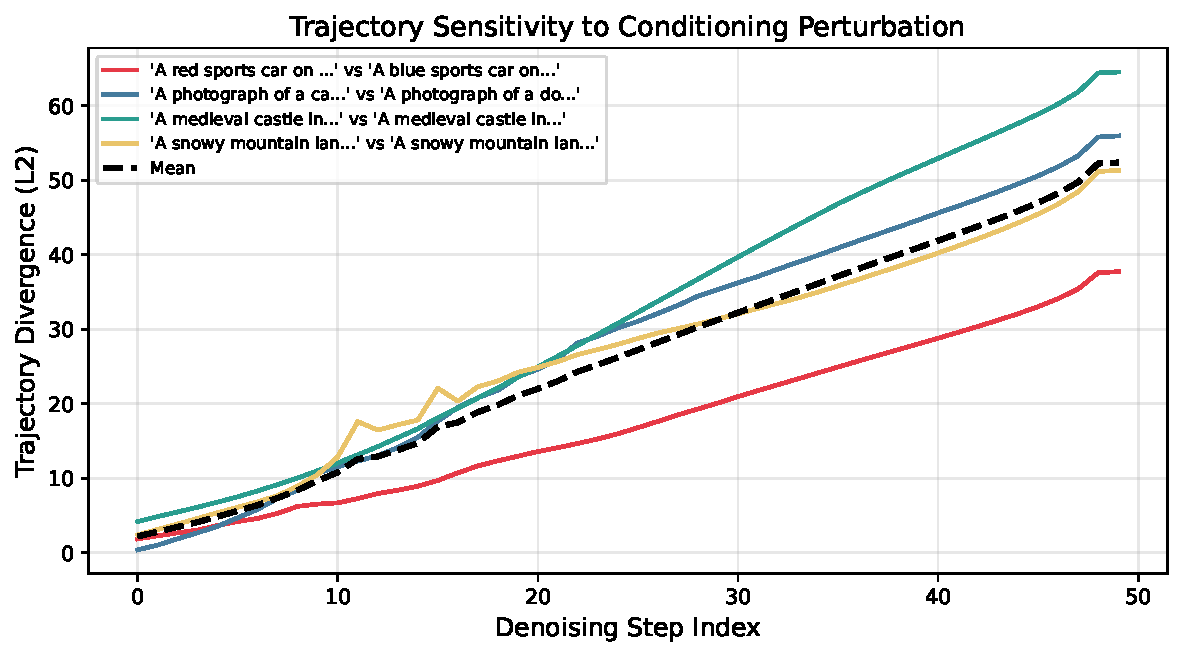
\includegraphics[width=\textwidth]{figures/sd15/trajectory_sensitivity.pdf}
        \caption{Cumulative TS.}
        \label{fig:ts}
    \end{subfigure}\hfill
    \begin{subfigure}[t]{0.32\textwidth}
        \centering
        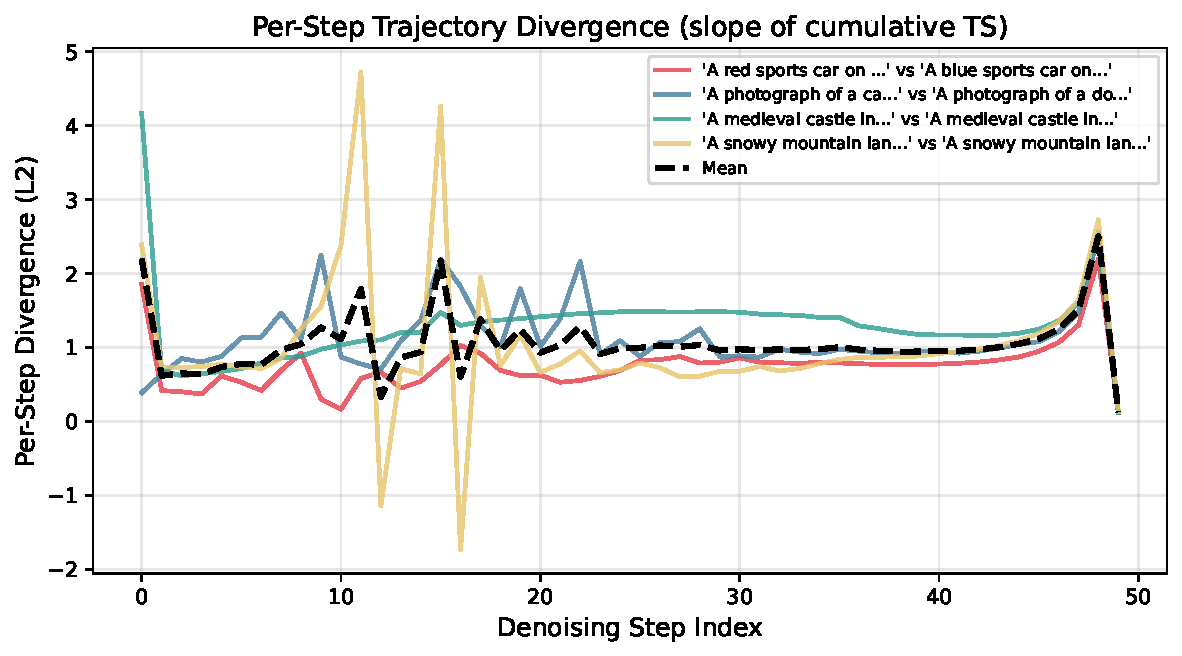
\includegraphics[width=\textwidth]{figures/sd15/trajectory_sensitivity_per_step.pdf}
        \caption{Per-step $\Delta$TS.}
        \label{fig:ts_per_step}
    \end{subfigure}\hfill
    \begin{subfigure}[t]{0.32\textwidth}
        \centering
        
\includegraphics[width=\textwidth]{figures/sd15/sas_curve.pdf}
        \caption{SAS across steps.}
        \label{fig:sas}
    \end{subfigure}
    \caption{SD~1.5 text conditioning: (a)~Cumulative trajectory divergence grows monotonically. (b)~Per-step divergence peaks in the early-to-mid phase. (c)~Semantic alignment plateaus by mid-phase.}
    \label{fig:ts_sas}
\end{figure}

% ---------------------------------------------------------------------------
\subsection{Structural Conditioning: CIS and SAS}

Figure~\ref{fig:struct_cis_sas} presents structural CIS and SAS for SD~1.5. The structural CIS peaks later (step~43) than text CIS (step~24) and reaches much higher magnitudes (mean peak 26.1 vs.\ 3.2), indicating that ControlNet's spatial residuals exert progressively stronger influence as the image crystallizes and finer structural details become resolvable.

The structural SAS (edge IoU) rises from near zero and grows most steeply in the mid-to-late phase, while the accompanying text SAS (measured via CLIP) rises earlier and plateaus sooner. This confirms a \textbf{temporal decoupling}: text conditioning shapes semantic content first, while structural conditioning refines spatial layout afterwards.

\begin{figure}[t]
    \centering
    \begin{subfigure}[t]{0.48\textwidth}
        \centering
        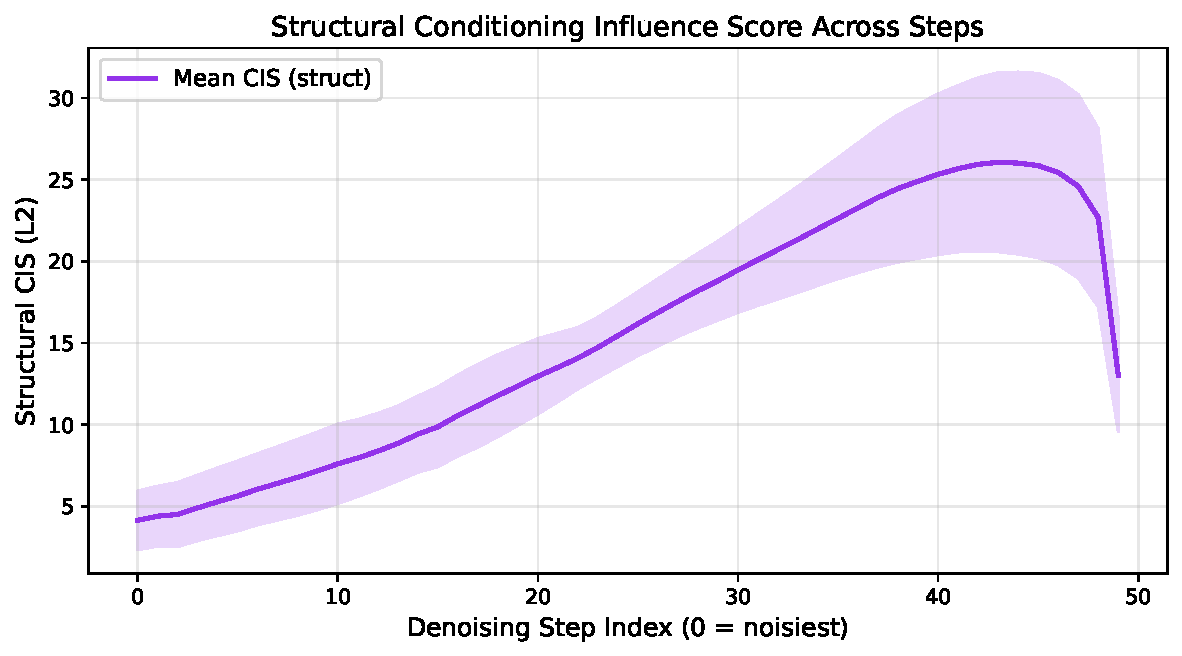
\includegraphics[width=\textwidth]{figures/sd15/cis_struct_curve.pdf}
        \caption{Structural CIS across denoising steps.}
        \label{fig:cis_struct}
    \end{subfigure}\hfill
    \begin{subfigure}[t]{0.48\textwidth}
        \centering
        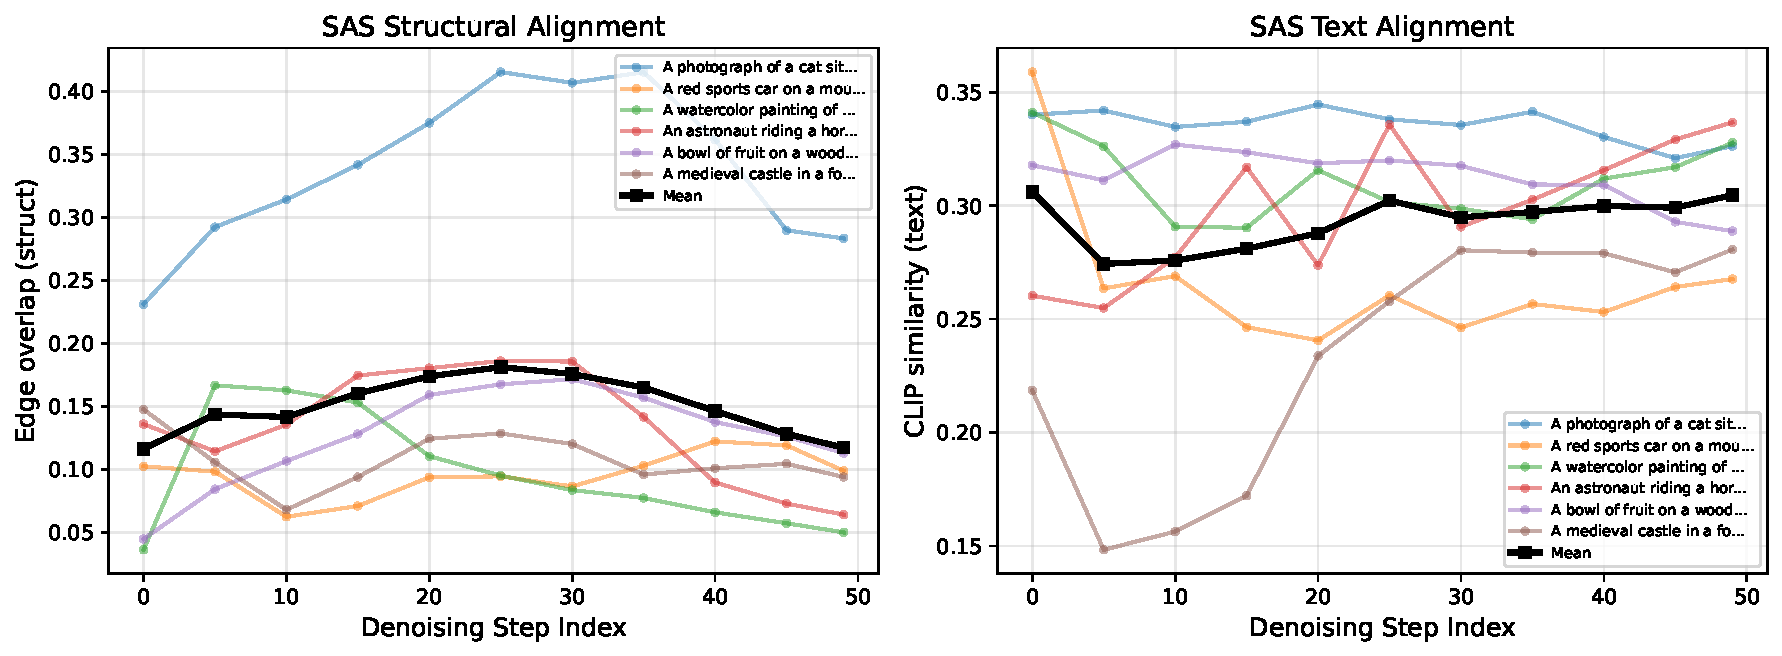
\includegraphics[width=\textwidth]{figures/sd15/sas_struct_curves.pdf}
        \caption{Structural SAS (edge IoU) and text SAS (CLIP).}
        \label{fig:sas_struct}
    \end{subfigure}
    \caption{SD~1.5 structural conditioning. (a)~Structural CIS peaks later and higher than text CIS, showing ControlNet influence grows as images crystallize. (b)~Edge alignment grows in mid-to-late steps while text alignment plateaus earlier, revealing temporal decoupling of the two modalities.}
    \label{fig:struct_cis_sas}
\end{figure}

\subsection{Structural Conditioning: Trajectory Sensitivity}

Figure~\ref{fig:ts_struct} shows the structural TS for SD~1.5. Pairs of different control images (same text prompt, same initial noise) produce trajectories that diverge more rapidly and to a greater final extent (mean final divergence: 62.5) than text-only pairs (52.4). This indicates that structural perturbations propagate more aggressively through the denoising process, consistent with ControlNet's direct injection into UNet residuals at every layer.

\begin{figure}[t]
    \centering
    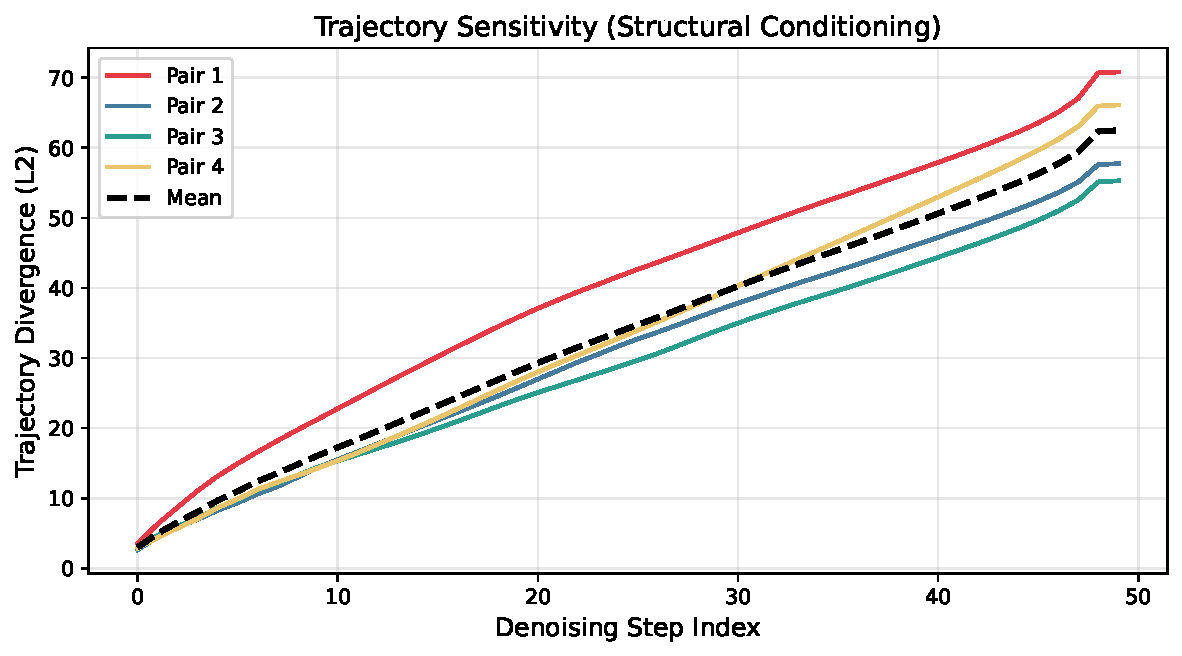
\includegraphics[width=0.48\textwidth]{figures/sd15/ts_struct.pdf}
    \caption{SD~1.5: Structural TS divergence for different control image pairs (same prompt, same noise). Final divergence is higher than text TS, indicating structural perturbations propagate more aggressively.}
    \label{fig:ts_struct}
\end{figure}

\subsection{Structural Conditioning: Selective Intervention}

Table~\ref{tab:selective_struct} reports edge IoU and CLIP scores under selective structural conditioning for both models. For SD~1.5, full structural conditioning achieves the highest edge IoU (0.124), and early-only conditioning drops sharply (0.039), comparable to no conditioning (0.038). Late-only conditioning recovers moderate structural fidelity (0.089), while mid-only falls between (0.067). This ordering---\emph{full $>$ late $>$ mid $>$ early $\approx$ none}---contrasts with text conditioning where \emph{mid} is most impactful, and reveals that structural fidelity depends more on later denoising steps where spatial details are being finalized.

For SDXL, the same trend holds with larger magnitudes: full conditioning achieves 0.410 edge IoU (vs.\ 0.124 for SD~1.5), consistent with SDXL ControlNet's stronger structural adherence. CLIP scores remain high across all windows because text CFG is always active; the variation reflects only the indirect effect of structural conditioning on semantic coherence.

\begin{table}[t]
\centering
\small
\caption{Selective structural conditioning: edge IoU (Struct) and CLIP scores. Bold marks best Struct per model.}
\label{tab:selective_struct}
\vspace{2pt}
\begin{tabular}{@{}llccccc@{}}
\toprule
Model & Metric & Full & Early & Mid & Late & None \\
\midrule
\multirow{2}{*}{SD 1.5}
& Struct IoU  & \textbf{0.124} & 0.039 & 0.067 & 0.089 & 0.038 \\
& CLIP score  & 0.315 & 0.270 & 0.296 & 0.268 & 0.259 \\
\midrule
\multirow{2}{*}{SDXL}
& Struct IoU  & \textbf{0.410} & 0.100 & 0.074 & 0.117 & 0.047 \\
& CLIP score  & 0.266 & 0.267 & 0.306 & 0.319 & 0.322 \\
\bottomrule
\end{tabular}
\end{table}

% ---------------------------------------------------------------------------
\subsection{Cross-Model Comparison: SD~1.5 vs.\ SDXL}

Our experiments reveal several consistent trends and informative differences between SD~1.5 and SDXL:

\paragraph{Consistent trends.}
(1)~Text CIS peaks at the same relative position (around step~24) with similar magnitudes (3.17 vs.\ 3.29). (2)~Structural CIS is an order of magnitude larger than text CIS in both models. (3)~SAS rises rapidly in early steps and plateaus by mid-phase in both models.

\paragraph{Key differences.}
(1)~\textbf{SDXL front-loads text conditioning}: early-only CLIP (0.311) nearly matches full (0.322), while SD~1.5 shows a larger gap (0.151 vs.\ 0.281). This is visible in SDXL's selective text results where mid/late/none conditions collapse to near-identical low scores. (2)~\textbf{SDXL amplifies structural effects}: SDXL achieves $3.3\times$ higher structural IoU under full conditioning (0.410 vs.\ 0.124). (3)~\textbf{Higher trajectory divergence}: SDXL produces larger final TS values for both text (73.4 vs.\ 52.4) and structural (117.8 vs.\ 62.5) perturbations, suggesting its larger capacity leads to more differentiated generation paths.

Figure~\ref{fig:sdxl_comparison} shows the SDXL counterparts of the SD~1.5 CIS results, confirming these trends visually.

\begin{figure}[t]
    \centering
    \begin{subfigure}[t]{0.48\textwidth}
        \centering
        
\includegraphics[width=\textwidth]{figures/sdxl/cis_curve.pdf}
        \caption{SDXL: Text CIS across steps.}
        \label{fig:sdxl_cis}
    \end{subfigure}\hfill
    \begin{subfigure}[t]{0.48\textwidth}
        \centering
        
\includegraphics[width=\textwidth]{figures/sdxl/cis_struct_curve.pdf}
        \caption{SDXL: Structural CIS across steps.}
        \label{fig:sdxl_cis_struct}
    \end{subfigure}
    \caption{SDXL conditioning influence scores. Text CIS (a) peaks early with similar magnitude to SD~1.5. Structural CIS (b) peaks at step~17 (earlier than SD~1.5's step~43), suggesting SDXL ControlNet concentrates structural influence in earlier steps.}
    \label{fig:sdxl_comparison}
\end{figure}

% ---------------------------------------------------------------------------
\subsection{Adaptive Guidance Schedule}

Motivated by our finding that text conditioning influence concentrates in the early-to-mid phase, we evaluate whether a \emph{time-dependent} guidance schedule can reduce computation while preserving semantic quality. We compare five schedules on SD~1.5 (Table~\ref{tab:adaptive}):

\begin{itemize}[nosep, leftmargin=*]
    \item \textbf{Uniform} ($w{=}7.5$ at all steps): the standard baseline.
    \item \textbf{Early-heavy} ($w{=}15$ for 0--40\%, $w{=}3$ thereafter): aggressively front-loads guidance.
    \item \textbf{Mid-heavy} ($w{=}3$/$15$/$3$ for early/mid/late): concentrates guidance in the mid phase.
    \item \textbf{Truncated 70\%} ($w{=}7.5$ for 0--70\%, $w{=}1$ thereafter): disables CFG in the late phase where CIS is low.
    \item \textbf{Linear decay} ($w$ linearly decreases from 7.5 to 1.5): smoothly tapers guidance.
\end{itemize}

\begin{table}[t]
\centering
\small
\caption{Adaptive guidance schedule comparison (SD~1.5). UNet calls counts the total forward passes; truncating CFG in late steps saves 15\% compute. Bold marks the best non-uniform schedule.}
\label{tab:adaptive}
\vspace{2pt}
\begin{tabular}{@{}lccc@{}}
\toprule
Schedule & Mean CLIP & UNet Calls & Relative Cost \\
\midrule
Uniform ($w{=}7.5$)       & \textbf{0.281} & 100 & 100\% \\
Early-heavy (15/3)        & $-$0.001 & 100 & 100\% \\
Mid-heavy (3/15/3)        & 0.217 & 100 & 100\% \\
Truncated 70\%            & \textbf{0.264} & 85  & 85\% \\
Linear decay              & 0.255 & 100 & 100\% \\
\bottomrule
\end{tabular}
\end{table}

The truncated schedule achieves 94\% of the uniform CLIP score while reducing UNet forward passes by 15\%, confirming that late-stage CFG contributes minimally to semantic content. In contrast, the early-heavy schedule catastrophically degrades quality (CLIP $\approx 0$), demonstrating that \emph{excessive} early guidance without sustained mid-phase reinforcement is harmful. The mid-heavy and linear decay schedules perform reasonably but do not offer compute savings. These results validate our CIS-based insight: guidance resources are most efficiently allocated to the early-to-mid phase, and late-phase CFG can be safely reduced.

% ===========================================================================
\section{Discussion}
\label{sec:discussion}
% ===========================================================================

\paragraph{Temporal decoupling of conditioning modalities.}
Our most notable finding is the temporal separation between text and structural conditioning influence. Text conditioning peaks in the early-to-mid phase and shapes semantic content, while structural conditioning peaks later and primarily governs spatial layout. Our adaptive schedule experiment (Section~\ref{sec:results}) validates this: truncating text CFG after 70\% of steps retains 94\% of semantic quality while saving 15\% of UNet forward passes, demonstrating that CIS-informed schedules can improve efficiency without sacrificing quality.

\paragraph{Model scale effects.}
SDXL's tendency to front-load text conditioning (early-only matching full) implies that larger models resolve semantic content faster. This has practical implications: SDXL may tolerate more aggressive early truncation of CFG without quality loss, potentially reducing inference cost.

\paragraph{Novelty and advantages.}
This work provides the first systematic, quantitative framework for measuring conditioning effectiveness across noise levels, modalities, and model scales. The three metrics (CIS, TS, SAS) are model-agnostic and require no retraining. The consistency of our findings across two model families and two conditioning types suggests generalizability beyond the specific architectures studied.

\paragraph{Limitations.}
Our analysis is limited to inference-time behavior and does not explain why certain noise-level dependencies arise during training. The CLIP-based SAS metric inherits known biases of CLIP~\citep{radford2021learning}, including reduced sensitivity to spatial relationships. The structural SAS (edge IoU) is a coarse measure of alignment that may miss fine-grained structural correspondence. We evaluate only DDIM sampling; other schedulers (e.g., DPM-Solver, Euler) may exhibit different temporal profiles. Finally, our ControlNet experiments use Canny edges only; other structural conditions (depth, pose) may show different noise-level dependencies.

% ===========================================================================
\section{Conclusion}
\label{sec:conclusion}
% ===========================================================================

We presented a measurement framework for quantifying how conditioning effectiveness varies across the reverse diffusion process. Through three complementary metrics (CIS, TS, SAS) and selective conditioning interventions, we characterized the noise-level dependence of both text and structural conditioning in SD~1.5 and SDXL. Our key findings are:

\begin{enumerate}[nosep, leftmargin=*]
    \item \textbf{Text conditioning peaks in the early-to-mid denoising phase} and shapes semantic content, with the CIS profile consistent across guidance scales and model families.
    \item \textbf{Structural conditioning peaks later} than text conditioning and primarily governs spatial layout, revealing a natural temporal decoupling between the two modalities.
    \item \textbf{Larger models front-load conditioning effects}: SDXL concentrates text conditioning influence in fewer early steps and achieves stronger structural adherence, suggesting that model scale changes the temporal dynamics of conditioning.
    \item \textbf{Selective conditioning confirms phase-specific roles}: removing conditioning from specific phases has modality-dependent effects---text quality degrades most without mid-phase CFG, while structural fidelity degrades most without late-phase ControlNet.
\end{enumerate}

These findings, together with our adaptive schedule experiment showing that CIS-informed truncation retains 94\% quality at 85\% cost, provide both principled understanding and practical tools for more efficient inference-time control in conditional diffusion models.

% ===========================================================================
\bibliographystyle{plainnat}
\begin{thebibliography}{10}

\bibitem[Ho et~al.(2020)]{ho2020denoising}
Jonathan Ho, Ajay Jain, and Pieter Abbeel.
\newblock Denoising diffusion probabilistic models.
\newblock In \emph{Advances in Neural Information Processing Systems (NeurIPS)}, 2020.

\bibitem[Song et~al.(2021a)]{song2021denoising}
Jiaming Song, Chenlin Meng, and Stefano Ermon.
\newblock Denoising diffusion implicit models.
\newblock In \emph{International Conference on Learning Representations (ICLR)}, 2021.

\bibitem[Song et~al.(2021b)]{song2021scorebased}
Yang Song, Jascha Sohl-Dickstein, Diederik~P. Kingma, Abhishek Kumar, Stefano Ermon, and Ben Poole.
\newblock Score-based generative modeling through stochastic differential equations.
\newblock In \emph{International Conference on Learning Representations (ICLR)}, 2021.

\bibitem[Rombach et~al.(2022)]{rombach2022high}
Robin Rombach, Andreas Blattmann, Dominik Lorenz, Patrick Esser, and Bj\"{o}rn Ommer.
\newblock High-resolution image synthesis with latent diffusion models.
\newblock In \emph{Proceedings of the IEEE/CVF Conference on Computer Vision and Pattern Recognition (CVPR)}, pages 10684--10695, 2022.

\bibitem[Ho and Salimans(2022)]{ho2022classifier}
Jonathan Ho and Tim Salimans.
\newblock Classifier-free diffusion guidance.
\newblock \emph{arXiv preprint arXiv:2207.12598}, 2022.

\bibitem[Hertz et~al.(2022)]{hertz2022prompt}
Amir Hertz, Ron Mokady, Jay Tenenbaum, Kfir Aberman, Yael Pritch, and Daniel Cohen-Or.
\newblock Prompt-to-prompt image editing with cross attention control.
\newblock In \emph{International Conference on Learning Representations (ICLR)}, 2023.

\bibitem[Zhang et~al.(2023)]{zhang2023adding}
Lvmin Zhang, Anyi Rao, and Maneesh Agrawala.
\newblock Adding conditional control to text-to-image diffusion models.
\newblock In \emph{Proceedings of the IEEE/CVF International Conference on Computer Vision (ICCV)}, 2023.

\bibitem[Radford et~al.(2021)]{radford2021learning}
Alec Radford, Jong~Wook Kim, Chris Hallacy, Aditya Ramesh, Gabriel Goh, Sandhini Agarwal, Girish Sastry, Amanda Askell, Pamela Mishkin, Jack Clark, Gretchen Krueger, and Ilya Sutskever.
\newblock Learning transferable visual models from natural language supervision.
\newblock In \emph{International Conference on Machine Learning (ICML)}, 2021.

\bibitem[Podell et~al.(2023)]{podell2023sdxl}
Dustin Podell, Zion English, Kyle Lacey, Andreas Blattmann, Tim Dockhorn, Jonas M\"{u}ller, Joe Penna, and Robin Rombach.
\newblock SDXL: Improving latent diffusion models for high-resolution image synthesis.
\newblock In \emph{International Conference on Learning Representations (ICLR)}, 2024.

\end{thebibliography}

\end{document}
